\chapter{Architecture}

\label{ch:architecture}

\section{Description}
	\subsection{Overview}
    
    	The dialogue chain is made of five modules: ASR, NLU, DM, NLG and TTS (Chap. \ref{ch:stateofart}). In the architecture introduced here, they are split in two groups: those forming the \textit{client} and those constituting the \textit{service}. The ASR and the TTS are necessarily included in the client and the  DM in the service. The NLU and the NLG can fit in both categories. This terminology has been borrowed to the computer network field where the client can refer to the user and to the application that interacts directly with the user in order to gather useful data for the interaction at the same time. Similarly, the server refers to the application that is in charge of handling user's requests, as well as the remote machine it is deployed on. In the case of dialogue systems, both parts can be embedded in the same device and they can also be distributed in two machines.
        
        Viewing traditional dialogue systems from this point of view translates into a ping-pong game, where the client sends a request which is processed by the service, and the latter sends a response back. The question we ask ourselves here is how to break this rigid mechanism in order to make the system able to process the user's speech incrementally. This chapter shows how, by starting from this new view of dialogue systems instead of the sequential one (dialogue chain), an incremental dialogue system can be derived from a traditional one at minimal cost. Moreover, in the resulting architecture, the turn-taking decision center is separated from the DM.
        
        As illustrated in Fig. \ref{fig:archioverview}, a new interface is inserted between the client and the service \cite{Khouzaimi2014a}. We call this new module the \textit{Scheduler} (this denomination is borrowed from \cite{Laroche2010}). It can be deployed in the same machine as the client, as the service or in a dedicated server. The objective to make the set \{Scheduler+service\} behave like an incremental dialogue system from the clients point of view, without modifying the initial functioning of the service. By doing so, we provide a framework that can transform any dialogue system in its incremental version just by adding a new layer.
        
        This alternative way of designing incremental dialogue systems also has the advantage of clearly separating turn-taking management from the rest. As it will be seen along this thesis, turn-taking strategies will be implemented exclusively in the Scheduler (the rest of the system remaining the same). Our ultimate goal is to make this module learn optimal turn-taking behaviours by itself.
        
     	\begin{figure*}[t]
          \centering
          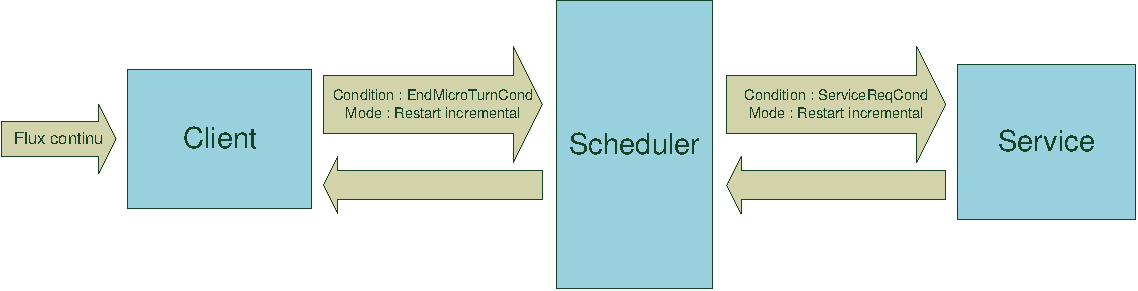
\includegraphics[scale=0.7]{figures/ClientSchedService.pdf}
          \caption{The Scheduler: an interface between the client and the service}
          \label{fig:archioverview}
        \end{figure*}
        
    \subsection{Time sharing}
    
    	There are four types of human machine interfaces, given whether both communication channels (from the user to the system and the other way around) are punctual or discrete:
        
        \begin{itemize}
        	\item \textbf{Discrete User/Discrete System:} This is the most basic way of human computer interaction. For example, the user hits a button and she immediately gets a response back. This is still widely used in many applications like browsers (when basic surfing, without watching videos or listening to audio).
            \item \textbf{Discrete User/Continuous System:} Most of the currently deployed vocal platforms operate in this mode as they asked the user for DTMF inputs while they use natural language to provide instructions (using pre-recorded audio or speech synthesis).
           	\item \textbf{Continuous User/Discrete System:} The application Shazam would be a good example of this communication mode. The user starts playing a song and the application listens. Once the latter recongnises it, it instantly displays the title and the singer on the screen.
            \item \textbf{Continuous User/Continuous System:} Spoken dialogue systems operate in a continuous/continuous mode. The communication signal from both sides is continuous.
        \end{itemize}
        
        For a system to be incremental, the user has to be continuous, therefore, the first and second communication modes are out of the scope of this thesis.
    
    	%HK> Revoir la construction du raisonnement (il faut que ce soit aussi rigoureux que dans le papier SigDial 2014).
    
    	In traditional dialogue systems, time is shared in a ordered and clear manner. The dialogue is a simple sequence of turns $T^1,T^2...$, a turn being the time interval in which a user's utterance followed by the system's response takes place, or the opposite (depending whether the system adopts a user initiative or a system initiative strategy at each time). For illustration and to simplify the notation, we will suppose that our system belongs to the first category, therefore, each turn is divided into two smaller time intervals, the user turn $T^{k,U}$ and the system turn $T^{k,S}$: $T^k = T^{k,U} \cup T^{k,S}$ (Fig. \ref{fig:timeshare}).
        
        In this chapter, a few conditions are defined to precisely describe time allocation between the system and the user. The \textit{activation time} of a condition refers to the exact moment when it goes from false to true. \textit{EndTurnCond} is the condition that ends a user turn, it is generally assimilated to a long silence \cite{Raux2008,Wlodarczak2013}.
        
        \begin{figure*}[t]
          \centering
          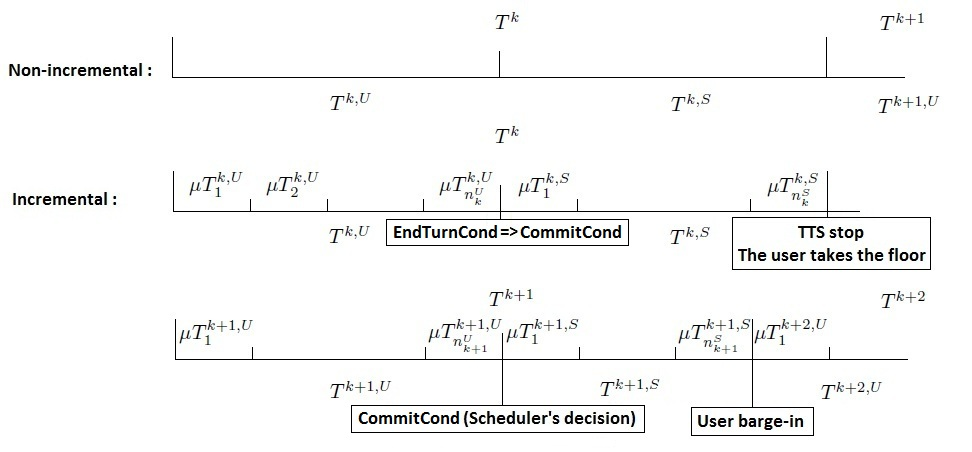
\includegraphics[scale=0.6]{figures/Timeline.jpg}
          \caption{Time sharing in traditional and incremental settings}
          \label{fig:timeshare}
        \end{figure*}
        
        In incremental settings, this time sharing formalism does not hold anymore and a new condition should be defined: \textit{EndMicroTurnCond} (with \textit{EndTurnCond} $\Rightarrow$ \textit{EndMicroTurnCond}). The time interval separating two activation times of \textit{EndMicroTurnCond} is called a \textit{micro-turn}. As a consequence, the turn $T^{k,U}$ can be divided into $n^{k,U}$ micro-turns $\mu T^{k,U}_i$: $T^{k,U} = \bigcup_{i=1}^{n^{k,U}} \mu T^{k,U}_i$. The $p^{th}$ \textit{sub-turn} of turn $T^{k,U}$ is defined as $T^{k,U}_p = \bigcup_{i=1}^p \mu T^{k,U}_i$.
        
        The request that user makes during $T^{k,U}$ is referred to as $Req^k$ and the corresponding response is $Resp^k$. This architecture does not process incremental units like in \cite{Schlangen2011}, instead, at each new micro-turn, it will take the whole information available since the beginning of the turn (at the $p^{th}$ micro-turn, all what the user uttered during $T^{k,U}_p$). This \textit{partial request} is called $Req^k_p$.
        
    \subsection{The Scheduler}
    
    	\begin{figure*}[ht]
          \centering
          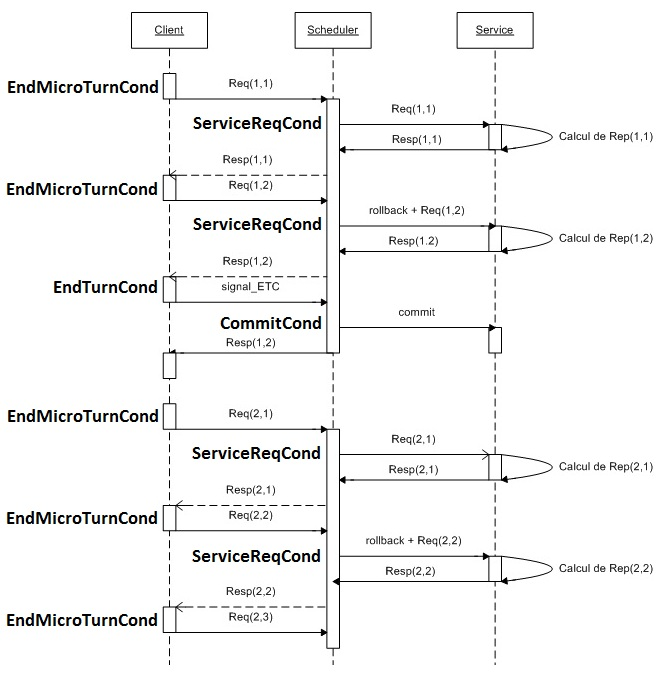
\includegraphics[scale=0.8]{figures/SchedChrono.jpg}
          \caption{Incremental behaviour with the Scheduler}
          \label{fig:schedchrono}
        \end{figure*}
    
    	During the $p^{th}$ micro-turn of the $k^{th}$ user turn, the client sends $Req^k_p$ to the Scheduler. The latter has to decide whether to send it to the service or not and the corresponding condition is called \textit{ServiceReqCond}. An good example is \textit{ServiceReqCond} = ($Req^k_p = Req^k_{p-1}$) as sending the same request twice is useless. Then, the service provides the corresponding response $Resp^k_p$ and the Scheduler stores it. The key idea of this architecture is that the Scheduler decides whether to retrieve this response to the client (making it take the floor through the TTS) or not (waiting for more information to come from the client. This decision can also be forced by the client when sending an end of turn signal $signal\_ETC$, like a long enough silence for instance. The most interesting fact about the Scheduler is that it is able to decide when to take the floor without waiting for $signal\_ETC$, the corresponding condition is called \textit{CommitCond}. The Scheduler functioning of over time is illustrated in Fig. \ref{fig:schedchrono}.
        
        \begin{figure*}[ht]
          \centering
          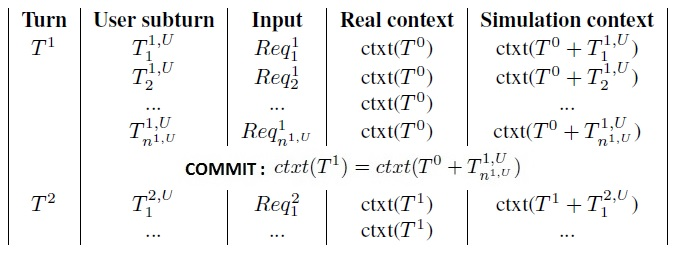
\includegraphics[scale=0.8]{figures/ContextChrono.jpg}
          \caption{Double context management: real and simulated}
          \label{fig:contextchrono}
        \end{figure*}
        
        Nevertheless, this approach raises on technical problem. Most of the requests that are made to the service are only aimed to see what would be its response for certain partial utterances and they are not used in the dialogue. However, they might modify the dialogue state in the service which is a side effect to be avoided. As a consequence, two dialogue contexts are maintained:
        
        \begin{itemize}
           	\item \textbf{The real context:} The dialogue context as traditionally used in dialogue systems. Contains the data and the variables that are aimed to last and be used in the rest of the dialogue.
        	\item \textbf{The simulated context:} A rough copy of the real context, at the $p^{th}$ micro-turn, $Resp^k_p$ could be useful for the dialogue or not. Therefore, only this context is modified at the first place, the Scheduler decides later whether to keep the changes in the real context or not.
        \end{itemize}
        
        These dialogue contexts are managed by two actions performed by the Scheduler:
        
        \begin{itemize}
        	\item \textbf{Commit:} The Scheduler commits to a partial request and the corresponding response when it decides to deliver the latter to the client, hence taking the floor immediately and not waiting for any further information. In that case, the simulated context is saved into the real context.
            \item \textbf{Cancel:} The scheduler cancels the context changes when it decides to discard the very last response obtained from the service. In that case, the real context is copied into the simulated one, rollbacking it to its original state. As shown in Fig \ref{fig:schedchrono}, this decision is only made when a new - potentially more complete - partial request is received from the client.
        \end{itemize}
 
 		The way the real and the simulated context are managed through the commit and the cancel actions is illustrated in Fig. \ref{fig:contextchrono}.

        
\section{Illustration}

	\subsection{A textual dialogue system: CFAsT}
    
    	\begin{figure*}[ht]
          \centering
          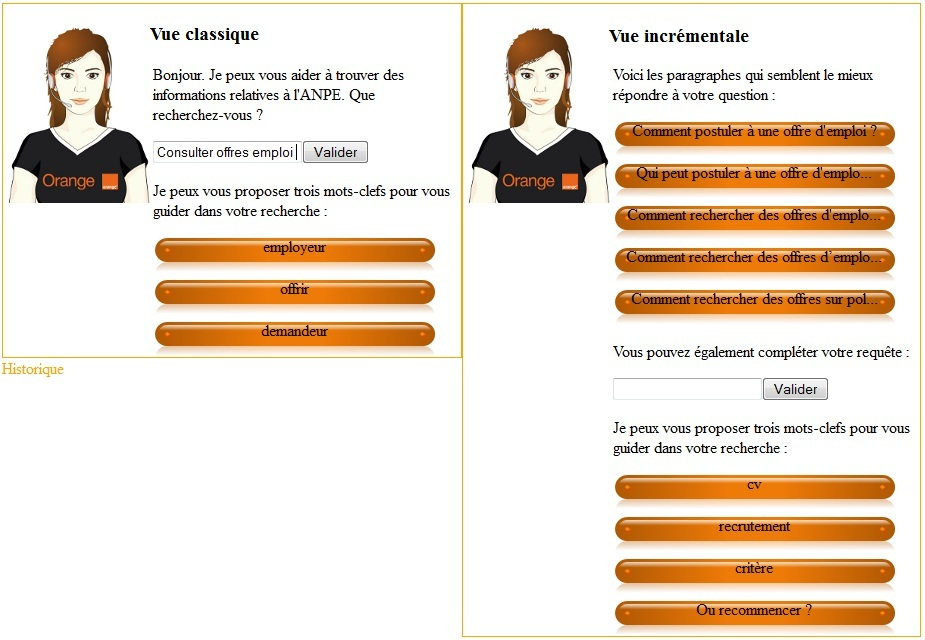
\includegraphics[scale=0.6]{figures/CFAsTIncr.jpg}
          \caption{The incremental version of the CFAsT project}
          \label{fig:CFAsTIncr}
        \end{figure*}
        
        CFAsT stands for Content Finder AssistanT. This application developed at Orange Labs is aimed to automatically generate a virutal assistant that helps the user to efficiently find a specific content in a database. At each dialogue turn, the user provides some new information about his target and by using a keyword spotting algorithm, the system keeps narrowing the set of possibilites. The interface is made of a text box with a \textit{validate} button. The dialogue service is deployed as a web service on a servlet container and the client is a javascript web page loaded on the user's browser.
        
        In order to make it incremental, another servlet has been deployed on the same container as the service and the javascript requests have been re-targeted toward it (the service is no longer directly visible by the client). Moreover, as discussed earlier, the dialogue context in the service have been duplicated. In this setup, \textit{EndTurnCond} corresponds to the event of clicking on \textit{validate} (or hitting the carriage return). A word-based micro-turn configuration has been implemented, therefore, \textit{EndMicroTurnCond} is the action of hitting the space bar. \textit{ServiceReqCond} is not useful here, hence, it is true all the time.
        
        This implementation is aimed to provide a first proof of concept of the methodology introduced here. However, $signal_{ETC}$ = \textit{CommitCond} = \textit{EndTurnCond} as the Scheduler never takes commit decisions by itself. Therefore, this is a very limited illustration.
    
    \subsection{A spoken dialogue system: Dictanum}
    
    	Number dictation is an activity that can be encountered in several kinds of tasks: phone number dictation, credit card...Analysing human conversations is such a situation shows that the number at hand is often broken into small pieces (a few digits each) and a confirmation follows each one of them. Therefore, the number is incrementally grounded so that in the case of a misunderstanding, only the last part dictated has to be repeated. Traditional dialogue systems behave differently as they ask the user to enter the whole number at once. This translates into long and tedious dialogues as only one little mistake is enough to make the user repeat the number from the beginning, often for several times. For example:
        
        \begin{dialogue}
        	\speak{SYSTEM} Welcome to the Dictanum service. Please dictate your number.
            \speak{USER} 01 45 65 79 98.
            \speak{SYSTEM} The dictated number is 01 45 67 79 98. Is that correct?
            \speak{USER} No.
            \speak{SYSTEM} Sorry. Let us try again. Please dictate your number.
            \speak{USER} 01 45 65 79 98.
            \speak{SYSTEM} The dictated number is 01 47 65 79 98. Is that correct?
            \speak{USER} No.
            \speak{SYSTEM} Sorry. Let us try again. Please dictate your number. \\
            $\left[...\right]$
            \speak{SYSTEM} The dictated number is 01 45 65 79 98. Is that correct?
            \speak{USER} Yes.
            \speak{SYSTEM} Thank you for using Dictanum. Bye.
        \end{dialogue}
        
        With incremental dialogue processing, it is possible to design a strategy that is closer to the human behaviour. To show that, a number dictation dialogue system called Dictanum has been implemented in our lab. It performs turn-based dialogue hence asking the user for the whole number at once. Here, the client is a web page displayed on the browser that uses Google API for both the ASR and the TTS tasks and the service is servlet deployed on a Tomcat container.
        
        Afterwards, the approach introduced here has been used to build the incremental version of the system (like in the case of the CFAsT application, the Scheduler has been deployed as a servlet on the same container as the service). To do so, two silence duration thresholds have been defined: the short silence threshold $\delta_s$ and the long one $\Delta_s$. \textit{EndMicroTurnCond} is triggered when a short silence is detected and similarly, \textit{EndTurnCond} corresponds to long silences. The system has been modified to detect these short silences and to deliver a feedback (repeating the last 4 digits) if detected. If the user ignores the feedback and keeps dictating his number, the system keeps on adding digits to his list, however, if the user starts his next utterance with \textit{No}, the feedback content is deleted from the number. Here is a dialogue example:
        
        \begin{dialogue}
        	\speak{SYSTEM} Welcome to the Dictanum service. Please dictate your number.
            \speak{USER} 01 45
            \speak{SYSTEM} 01 45
            \speak{USER} 65 79
            \speak{SYSTEM} 67 79
            \speak{USER} No, 65 79
            \speak{SYSTEM} Sorry, 65 79
            \speak{USER} 98
            \speak{SYSTEM} 98
            \speak{USER} ...
            \speak{SYSTEM} The dictated number is 01 45 65 79 98. Is that correct?
            \speak{USER} Yes.
            \speak{SYSTEM} Thank you for using Dictanum. Bye.
        \end{dialogue}
        
        Dictanum also offers the possibility for the user to interrupt the system during the final feedback, in order to make local corrections. To do that, this feedback is sent to the TTS in the following format: \textit{The dictated number is 01 <sep> 45 <sep> 65 <sep> 79 <sep> 98. Is that correct?}. The latter pronounces the sentence chunk after chunk (chunks are delimited using the separator \textit{<sep>}), each chunk lasting for the same number of micro-turns. This leads to the following kind of strategy:
        
        \begin{dialogue}
        	\speak{SYSTEM} The dictated number is: 01 45 67...
            \speak{USER} No, 65.
            \speak{SYSTEM} Sorry. The dictated number is 01 45 65 79 98. Is that right?
            \speak{USER} Yes.
            \speak{SYSTEM} Thank you for using Dictanum. Bye.
        \end{dialogue}
    
\section{Discussion}

	\subsection{Levels of incrementality}
    
    	Dialogue systems can be classified in four categories given the way they integrate incremental behaviour. The first category is made of traditional systems \cite{CLASSiCd64}. Then comes the second category where traditional systems locally simulate a few incremental behaviours. For instance, in \cite{El-Asri2014}, the system enumerates a list of options and the user selects the one that fits him best by uttering \textit{Yes} or \textit{Ok} for example (REF\_RAW in the taxonomy introduced in Chap. \ref{ch:taxonomy}). The architecture introduced in this thesis belongs to the third category where incremental behaviour is obtained based on modules that are innately non-incremental (the service in our case). Other examples are described in \cite{Selfridge2012a} and \cite{Hastie2013}. Finally, the fourth category is made of incremental dialogue systems that are constituted of fully-incremental modules. In \cite{Schlangen2011}, an abstract model for incremental architectures is presented where all the categories can fit, but the work that has been pursued by the authors and their research groups later on goes along with the spirit of this last category.
		
		Categories 2, 3 and 4 embed different features related to incremental behaviour as summarised in Fig. \ref{tab:incrclassif}.

	\subsection{Enhancing a traditional dialogue system's turn-taking abilities at a low cost}
    
      \begin{table*}[!ht]
      	\footnotesize
        \centering
        \begin{tabular}{|c|c|c|c|c|}
          \hline
          \textbf{Features}	& \textbf{Category 1} & \textbf{Category 2} & \textbf{Category 3} & \textbf{Category 4} \\
          \hline
          TTS interruption after input analysis & - & + & + & + \\
          \hline
          Link interruption time with TTS & - & + & + & + \\
          \hline
          User interruption by the system & - & - & + & + \\
          \hline
          Better reactivity & - & - & + & + \\
          \hline
          Optimal processing cost & - & - & - & + \\
          \hline
        \end{tabular}
        \caption{Available features for dialogue systems given the way they integrate incrementality}
        \label{tab:incrclassif}
      \end{table*}
    
    \subsection{Separating dialogue management from floor management}
    
    
    
    
    
    
    
    
    
    
    
    
    
    
    
    
    
    
